\documentclass[letterpaper,10pt,conference]{ieeeconf}
\IEEEoverridecommandlockouts
\overrideIEEEmargins
\usepackage{fontspec}
\setmainfont{Times New Roman}\setsansfont{Arial}\setmonofont{Menlo}
\usepackage{amsmath,amssymb,graphicx,booktabs,cite,url}
\graphicspath{{figures/}}
\title{\LARGE\bf Posture and Contact Geometry in Simple Hybrid Locomotion\\of an Articulated Arc-Leg Hexapod}
\author{\mbox{}}
\begin{document}
\maketitle\thispagestyle{empty}\pagestyle{empty}
\begin{abstract}
An articulated arc leg can combine rolling and stepping without a separate wheel actuator. The resulting design is useful only if its mobility justifies the required control. We investigate how much control can be removed while retaining flat-ground transport and stair ascent on one hexapod embodiment. For flat motion, periodic reindexing replaces conditional swing scheduling. For stairs, a fixed leading-joint posture and one common distal phase replace height-dependent settings. A paired 102-trial MuJoCo study separates contact shape, posture, and stair dimensions and requires rear-leg clearance followed by a supported halt. With a 2 ms step, the fixed arc controller succeeds in all six conditions at each of 100 and 150 mm riser heights; height-dependent settings add no successes. The matched closed-wheel model succeeds in five and zero conditions, respectively. However, one 150 mm wheel outcome changes at 1 ms, and neither geometry completes the 200 mm flight under the stricter endpoint. A separate 176-trial flat study likewise finds no transport advantage for conditional scheduling over periodic reindexing under common target-rate limits. The evidence identifies where simple mode-specific control suffices and where simulation sensitivity or incomplete transfer prevents a mobility claim.
\end{abstract}

\section{INTRODUCTION}
A mobile robot moving between floor segments and stairs must produce both sustained horizontal travel and discrete elevation changes. Articulated wheel-leg systems can address these demands through contact placement and rolling. Their additional joints, however, create a practical question: which motions require active coordination, and which can be produced by contact geometry under a simple command? A demonstration that a robot moves in several modes does not answer that question.

SCONE is a six-legged platform with three actuated joints per limb and a fixed C-shaped terminal frame. The distal joint serves both articulation and arc rotation, without an additional wheel motor or a mechanism that closes the arc into a circle. On flat terrain, different legs can roll or step within a common gait. On stairs, the limb posture changes the position of each arc axis relative to an edge. The same terminal frame can then encounter a tread, riser, or corner as its phase advances.

We study this embodiment through \emph{control removal}. On the floor, a periodic swing policy provides a simpler alternative to conditional reindexing. On stairs, we replace a height lookup by a fixed posture and a single phase shared by all six distal joints. Matched closed wheels test the contribution of contact shape; a neutral-posture condition tests the additional leading-joint rotation. This design separates three possible explanations for ascent: geometry, posture, and controller selection.

\begin{figure}[t]\centering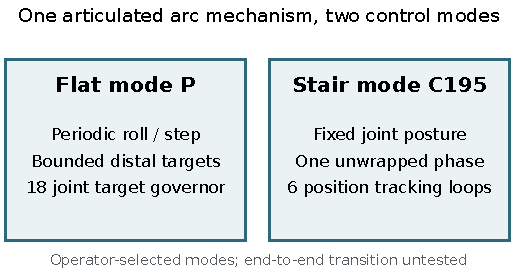
\includegraphics[width=\columnwidth]{hybrid_modes.pdf}
\caption{Evaluated mode-specific simplification. Flat motion uses periodic rolling/stepping allocation; stair motion uses a fixed acquired posture and a common distal phase. Each mode is tested separately. The experiments do not demonstrate autonomous terrain detection or an uninterrupted floor--stair--floor transition.}
\label{fig:modes}\end{figure}

The contributions are twofold. First, we formulate a restricted hybrid-control architecture that distinguishes bounded flat-mode reindexing from continuous stair-mode rotation. Its simplification concerns motion selection, not the number of hardware actuators. Second, we provide a paired mechanism study with explicit support and stopping criteria, retaining failed trials and numerical sensitivity. The study identifies a measured operating envelope for simple control, including incomplete rear-bank transfer and numerical sensitivity.

\section{RELATED WORK}
RHex established that curved legs and simple clock-driven gaits can provide substantial mobility~\cite{saranli2001rhex}. Q-Whex uses six actuators and sector-shaped quasi-wheels; its physical evaluation includes stairs with different phase patterns~\cite{zhang2023qwhex}. Thus, neither low-dimensional phase control nor curved-leg stair ascent is unique to SCONE. In particular, SCONE's eighteen actuators do not establish mechanical simplicity relative to Q-Whex. Our comparison asks whether the existing articulation requires height-specific coordination within a fixed embodiment.

Quattroped shares actuation between leg and wheel configurations~\cite{chen2014quattroped}; TurboQuad studies smooth behavioral transitions~\cite{chen2017turboquad}. ASTERISK H also combines leg and wheel locomotion~\cite{yoshioka2008asterisk}. These precedents motivate careful separation of shared actuation, shape transformation, and controller switching. SCONE retains an open terminal frame and changes limb posture and motion policy. We evaluate the policies separately and make no transition-performance claim.

Whole-body planning and control can coordinate rolling with articulated contact placement~\cite{bjelonic2019keep,bjelonic2021wholebody}. Such methods address forces and motion constraints beyond the position-based control studied here. We do not compare their performance across dissimilar hardware. Instead, we test whether additional scheduling is useful before introducing a more complex planner.

Rolling models also depend on the contact representation. Mane and Hubicki formulate rolling with planar parametric curves and smooth no-slip contact~\cite{mane2024rolling}. Our simulated stair contacts can slip and change between surfaces; a support tangent alone cannot certify edge traversal. Controlled testing is particularly important when small changes alter contact sequences~\cite{weng2024testing}. Accordingly, we report both matched contrasts and timestep sensitivity, rather than interpret a deterministic success count as field reliability.

\section{PROBLEM AND PLATFORM}
\subsection{Task and Scope}
The target use case consists of flat motion and ascent of a known stair flight. The mode is selected externally. The flat task measures transport and command tracking over a prescribed horizon. The stair task requires three risers to be crossed, followed by a supported stop on the top surface. A chassis that rises above the final edge while its rear bank remains below it has not completed this task.

Let $h$ denote riser height, $d$ tread depth, $R$ the terminal outer radius, $q_a$ the acquired limb posture, and $\phi$ a common distal phase. The question is whether one pair $(q_a,\dot\phi)$ preserves task completion across a specified set of $(h,d)$ and approach conditions. We test this empirically, with contact shape as a separate experimental factor. We do not infer a feasibility boundary from $h/R$ alone.

\subsection{Embodiment and Actuator Path}
The model mass is 4.161 kg. Each of the six limbs has a steering joint, a middle joint, and a distal joint carrying the terminal arc. The arc occupies approximately $225^\circ$ and has outer/inner radii of 122.5/112.5 mm and a width of 44 mm. The platform therefore shares the distal actuator between arc rotation and articulation, but retains eighteen actuators and their low-level feedback loops.

\begin{figure}[t]\centering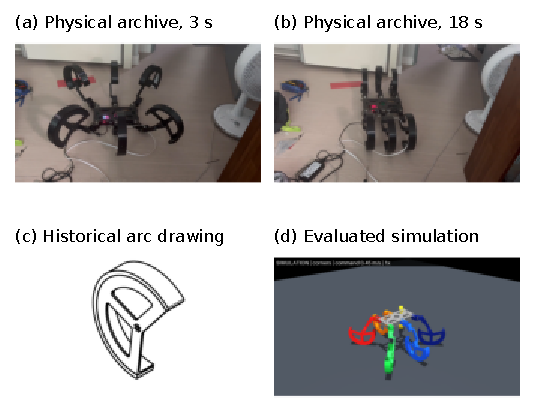
\includegraphics[width=\columnwidth]{platform.pdf}
\caption{SCONE embodiment and model. (a,b) Archival physical floor-motion frames at source times 3 and 18 s. (c) Historical fabrication drawing. (d) Simulation pose. Archival images document the mechanism; their undocumented controller and external cables prevent their use as validation of the evaluated policies.}
\label{fig:platform}\end{figure}

The simulated actuator path converts a position/velocity tracking error into a torque request and bounded motor voltage:
\begin{align}
 \tau_j^c&=k_{p,j}(q_j^\star-q_j)+k_{d,j}(\dot q_j^\star-\dot q_j),\\
 V_j&=\operatorname{sat}_{[-12,12]}[(R_j/K_j)\tau_j^c+K_j\dot q_j].
\end{align}
Reflected rotor inertia is included. The flat and stair modes retain their respective position-profile configurations; comparisons within each mode share gains and motor properties. We therefore compare control variants within a mode, rather than compare their measured energy across modes. No loaded actuator identification is available.

\subsection{Contact Geometry and Edge Interaction}
For an arc material point $c_i$, its world position can be expressed as
\begin{equation}
 p_i=o_i(q_a)+\mathcal{R}_i(q_a,\phi)c_i.
\end{equation}
Changing posture alters the axis location $o_i$ and orientation; changing the terminal shape alters the available contact points. A stair edge may consequently intersect different regions of the terminal frame under the same phase command. This is the proposed physical explanation to test, not a no-slip or stable-pivot guarantee.

The familiar single-wheel horizontal-push model becomes singular as a riser approaches the axle height. It does not establish impossibility for a powered, articulated multi-contact robot. We therefore use a matched closed-wheel comparison instead of an $h/R$ feasibility bound.

Ordinary mesh collision in MuJoCo uses a convex representation~\cite{mujococollision}. A single mesh can fill the visible arc cavity. Our primary arc model uses CoACD~\cite{wei2022coacd}, with 24 convex parts per tire, a 2 mm concavity threshold, and unchanged explicit body mass and inertia. A 1 mm probe at the axle center contacts the single hull but not the decomposition; the outer support-function difference over 720 directions is below 0.004 mm. The summed part volume exceeds the original mesh by 2.76\%, so the collision shape remains an approximation.

\begin{figure}[t]\centering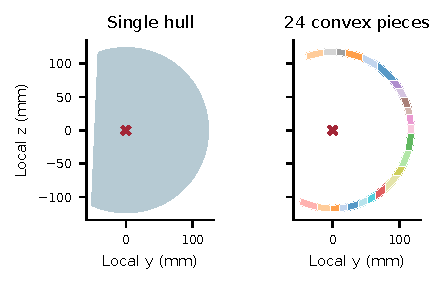
\includegraphics[width=\columnwidth]{collision.pdf}
\caption{Collision geometry used in the stair comparison. The single hull fills the cavity; the decomposed representation preserves it. The closed-wheel condition instead uses a cylinder with the same radius, width, mass, and inertia. The study compares complete shape representations, not an isolated inner-hook feature.}
\label{fig:collision}\end{figure}

\section{MODE-SPECIFIC CONTROL SIMPLIFICATION}
\subsection{Flat Motion: Periodic Reindexing}
A geometric allocator assigns rolling and stepping roles from the requested contact travel. Under forward motion, four legs roll while two step; steering and roles are held until a swing permits repositioning. Articulation receives the requested travel left after the commanded rolling increment. Numerical inverse kinematics produces joint targets.

We compare periodic reindexing (P) with a conditional policy (B). P gives each rolling leg a swing at every scheduled opportunity. B may skip a swing, using remaining angular reserve and a prediction to the next opportunity. Both apply a swing-time sector budget and a slew guard. A quintic return from a sector offset $\theta_0$ to home has peak rate $15|\theta_0|/(8T_s)$; limiting $|\theta_0|$ to $8\Omega T_s/15$ bounds that component. It does not bound the total distal target, which also contains inverse-kinematic motion.

A common governor limits changes in all eighteen issued targets. Let $q_k^d$ be a requested target, $q_k^I$ an issued target, and $\ell_j$ a per-update allowance. In encoder counts,
\begin{equation}
 q_{j,k+1}^I=q_{j,k}^I+\operatorname{clip}(q_{j,k}^d-q_{j,k}^I,-\ell_j,\ell_j).
\end{equation}
Quantized allowances and inner velocity profiles enforce the declared command bounds. The nominal group speeds are 330, 276, and 462 degree/s, derived from 12 V no-load specifications~\cite{robotisMX,robotisW350,robotisW210}; $\rho$ scales these values. In H, the gait clock waits until a requested target has been fully issued. In F, the clock continues, so intermediate requests can change. Neither waits for measured joint arrival. We select P as the simpler flat policy because the experiments do not show a transport benefit for B.

\subsection{Stairs: Fixed Posture and One Phase}
The stair policy first acquires a side-on posture through the existing scripted mode sequence. It then sets the three leading middle joints, motor IDs 7, 9, and 11, to $\alpha$. Other acquired proximal targets remain held. After all six distal joints acquire an initial phase, the policy advances one unwrapped variable:
\begin{align}
 \phi_{k+1}&=\phi_k-\omega u\Delta t,\\
 q_{3,i}^\star&=s_i\phi+b_i,\quad
 (s_i,b_i)=\begin{cases}(1,0),&i\ \text{odd},\\(-1,360^\circ),&i\ \text{even}.\end{cases}
\end{align}
Here $u\in[-1,1]$ is a normalized operator command. It controls phase rate, not measured chassis speed. Six independent position loops track this common command; unequal contact loads need not yield equal actual phases.

The fixed policy C195 uses $\alpha=195^\circ$, $\phi_0=90^\circ$, and $\omega=274.8^\circ$/s for every stair. C180 changes only $\alpha$ to $180^\circ$. The existing lookup CL selects $(180^\circ,60^\circ,343.5^\circ/\mathrm{s})$ at 100 mm, $(184^\circ,60^\circ,274.8^\circ/\mathrm{s})$ at 150 mm, and the C195 settings at 200 mm. CL uses known height before motion; it does not adapt online to contact or terrain. Removing its two height thresholds removes a configuration dependency, while retaining one phase state and six tracking loops.

Unlike bounded flat-mode targets, stair-mode extended-position commands permit multiple revolutions. A finite material arc does not itself require bounded shaft rotation. This distinction is essential: the flat rewind guarantee does not describe the stair controller, and the stair experiment does not validate physical multi-turn clearance or wiring.

\section{EXPERIMENTAL METHOD}
\subsection{Frozen Stair Comparison}
A 12-run exploratory test of existing nominal presets motivated C195. We then froze the source and the complete factorial design before running it. The grid is a deterministic sensitivity study; it is not a held-out population sample. MuJoCo 3.10.0~\cite{todorov2012mujoco} runs with a 2 ms physics step and 20 ms control update.

Each flight has three equal risers, $h\in\{100,150,200\}$ mm, equal treads $d\in\{250,350\}$ mm, 1 m width, and a 0.70 m landing after the third tread. Three initial approach offsets $(\Delta y,\Delta\psi)$ are $(0,0)$, $(-30\ \mathrm{mm},3^\circ)$, and $(30\ \mathrm{mm},-3^\circ)$. The latter cases combine translation and yaw and do not isolate their effects. Offsets are applied after scripted side-pose acquisition and before brace/phase acquisition, with velocity reset. There is no state reset during measured ascent.

The two geometries and two fixed postures yield $3\times2\times3\times2\times2=72$ paired trials. CL adds 18 arc trials. Twelve timestep checks repeat the fixed 195-degree policy for both geometries, all three heights, 350 mm treads, and nominal approach at 1 and 4 ms. The total is 102 trials. Geometry pairs preserve inertial properties, gains, rates, and posture commands. Actual acquired states can differ through contact dynamics. The shape contrast also changes contact topology and numerical representation; it cannot attribute an effect solely to inner-surface hooking.

\subsection{Completion and Timing}
Brace and phase acquisition each receive 4 s. Their respective tolerances are 256 and 96 encoder counts. Failure to acquire remains in the trial denominator. The scripted side-pose sequence takes approximately 23 s; it is not an optimized locomotion transition. We retain its time and work separately and include it in total task cost.

Ascent has a 20 s horizon. All six terminal centers must pass the final riser by at least $R$, and at least three distinct tire bodies must each have a contact above 1 N within 10 mm of the top height. The phase then stops. Within the next 2 s, the same clearance and support conditions must hold for 0.5 s, with root linear speed below 0.05 m/s and angular speed below 0.2 rad/s. These endpoint conditions are sampled at 50 Hz. A root-up component below 0.5 at any physics step terminates ascent or halt. The test checks a supported stop, not a positive static stability margin.

We report ascent completion and supported halt separately. Absolute mechanical work is $\int\sum_j|\tau_j\dot q_j|dt$, not battery energy. Time-to-ascent excludes acquisition; total time includes acquisition and halt. Failed horizons are retained but are not averaged into successful time-to-top values. The design does not estimate hardware failure probabilities.

\subsection{Complementary Flat Study}
A separate frozen 176-trial design compares the original allocator U, conditional B, and periodic P with the same arc model and flat-mode gains. It uses four initial phases, two forward commands (0.18 and 0.45 m/s), and 20 s main trials under unlimited targets, H at $\rho=1.0$ and 0.8, and F at $\rho=0.8$ (96 trials). H at $\rho=0.5$ adds 12 high-command trials. Forward--stop--reverse and turning sequences add 48 trials of 24 s. Twelve runs last 60 s, and eight repeat selected high-command B/P cases at 1 or 4 ms.

Forward speed is displacement along the initial body axis divided by the observation duration. Root-point velocity integration provides an independent check. Joint tracking RMS, requested-to-issued lag, and loaded-contact counts expose costs hidden by target-rate compliance. The flat and stair studies use different preparation and success rules; their counts and work are not pooled.

\section{RESULTS}
\subsection{What the Fixed Stair Policy Retains}
All 102 trials acquire the prescribed posture and phase without exception; 53 reach the supported-halt endpoint and 49 time out during ascent. In this grid, every trial that satisfies the ascent criterion also achieves the subsequent halt. Table~\ref{tab:stairs} reports the 90 main-grid trials, with timestep checks kept separate.

\begin{table}[t]\centering\small
\caption{Supported halt after three steps, 2 ms physics step}
\label{tab:stairs}\begin{tabular}{lccc}\toprule
 & 100 mm & 150 mm & 200 mm\\\midrule
C195 & 6/6 & 6/6 & 0/6\\
C180 & 6/6 & 6/6 & 0/6\\
CL & 6/6 & 6/6 & 0/6\\
W195 & 5/6 & 0/6 & 0/6\\
W180 & 5/6 & 0/6 & 0/6\\
\bottomrule\end{tabular}
\par\vspace{4pt}\noindent\parbox{\columnwidth}{\footnotesize Six conditions per cell: two tread depths and three approach poses. C/W denote decomposed arcs/closed wheels. 195/180 are fixed leading-joint angles; CL uses the height lookup. These are deterministic condition counts.}
\end{table}
\begin{table}[t]\centering\small
\caption{Ascent cost among successful arc trials, 2 ms}
\label{tab:cost}\begin{tabular}{ccccc}\toprule
Rise & Code & Ascent (s) & Work (J) & Total (s)\\\midrule
100 & C195 & 4.04 & 75.6 & 35.77\\
100 & C180 & 4.08 & 76.3 & 35.75\\
100 & CL & 3.41 & 63.5 & 35.33\\
150 & C195 & 5.41 & 105.3 & 37.11\\
150 & C180 & 6.41 & 119.3 & 38.11\\
150 & CL & 5.29 & 96.4 & 36.97\\
\bottomrule\end{tabular}
\par\vspace{4pt}\noindent\parbox{\columnwidth}{\footnotesize Means over the same six successful conditions per row. Work is absolute actuator mechanical work during ascent. Total time includes scripted pose acquisition, 8 s of brace/phase acquisition, ascent, and stable halt.}
\end{table}

At 2 ms, C195 completes all six conditions at 100 mm and all six at 150 mm. C180 and CL achieve the same counts. The 150 mm result corresponds to $h/R=1.22$, but that ratio is descriptive, not a feasibility proof. Height selection adds no successful conditions to this grid. Its timing can still matter: at 100 mm, CL ascends in 3.41 s on average, compared with 4.04 s for C195; at 150 mm, the corresponding values are 5.29 and 5.41 s.

\begin{figure*}[t]\centering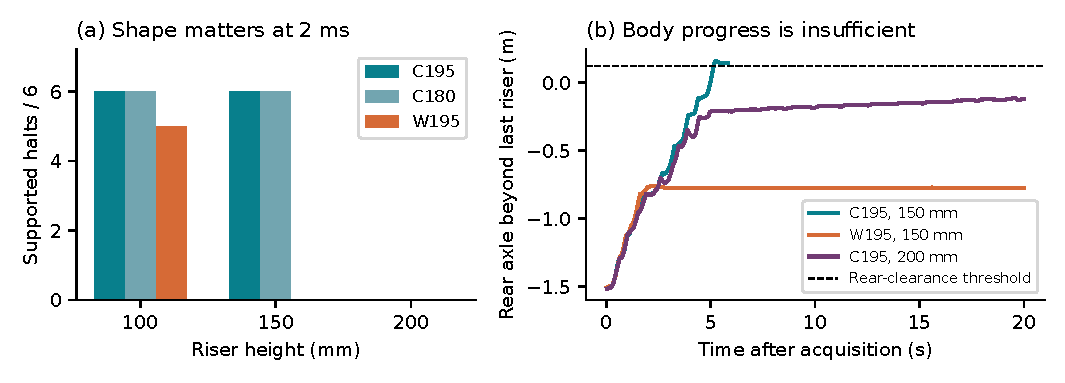
\includegraphics[width=.98\textwidth]{stair_overview.pdf}
\caption{Measured stair outcomes and clearance. (a) Main-grid supported halts at 2 ms. (b) Nominal 350 mm-tread replays show the rearmost terminal center relative to the final riser. Passing the dashed line is necessary but not sufficient: loaded top contacts and a stable halt are also required. At 200 mm the chassis progresses while the rear bank remains below the clearance threshold. The closed-wheel 150 mm outcome changes at 1 ms and is not a geometry-independent impossibility result.}
\label{fig:results}\end{figure*}

The posture comparison gives a narrower benefit than a new capability. At 150 mm, C195 reduces mean ascent time from C180's 6.41 s to 5.41 s and absolute work from 119.3 to 105.3 J. Both still succeed in the same six conditions. At 100 mm, ascent times are nearly equal. Thus the additional $15^\circ$ posture change helps transport cost in the tested 150 mm cases, but is not necessary for their completion. Including scripted preparation increases mean total time to approximately 35--38 s (Table~\ref{tab:cost}); quoting ascent alone would conceal most of this implementation's task time.

\subsection{Contact Shape, Failure, and Numerical Sensitivity}
At 2 ms, W195 and W180 each complete five of six 100 mm conditions and none of the six 150 mm conditions. The matched arc outcome supports a contact-shape advantage under this discretization and controller, with no corresponding evidence that a height lookup is required. Figure~\ref{fig:replay} shows nominal motion under the same phase command.

\begin{figure*}[t]\centering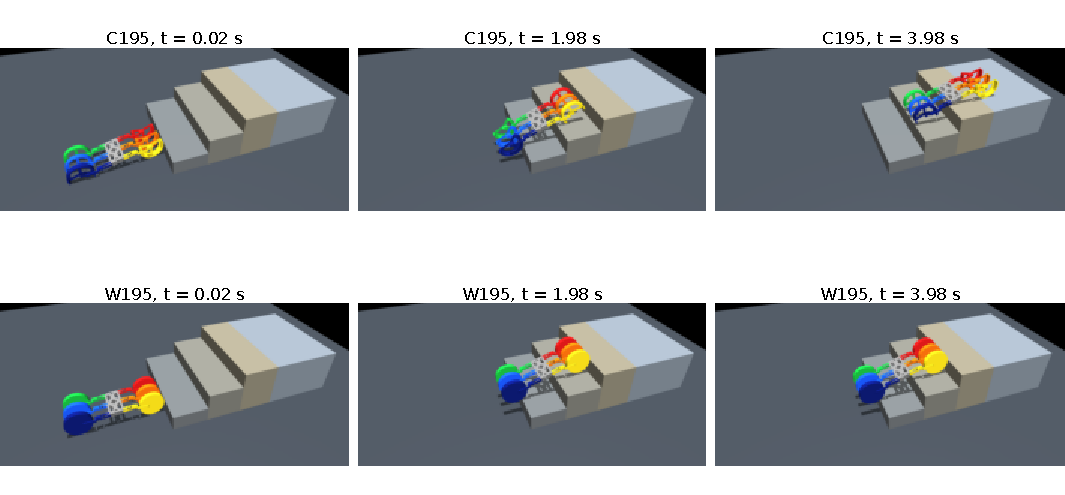
\includegraphics[width=.98\textwidth]{stair_replay.pdf}
\caption{Independent replays at 150 mm rise, 350 mm tread, nominal approach, and 2 ms physics step. C195 (top) advances through the flight; W195 (bottom) remains near the lower steps. Images show actual simulated states with a fixed camera. Replayed numerical endpoints and work match the original trial records exactly. The matched wheel succeeds at 1 ms, so these images illustrate the reported 2 ms contrast only.}
\label{fig:replay}\end{figure*}

The timestep study limits that interpretation. C195 retains nominal success at 100 and 150 mm and failure at 200 mm at all three steps. W195 succeeds at 100 mm and fails at 200 mm throughout, but its nominal 150 mm trial succeeds at 1 ms and fails at 2 and 4 ms. Preparation also evolves at the selected step, so this check measures end-to-end numerical sensitivity rather than isolating integration error from one identical acquired state. A universal claim that the closed-wheel geometry cannot climb these stairs is unsupported.

None of the 30 main-grid trials at 200 mm meets the full ascent criterion. Some raise the chassis close to the top while leaving the rear bank on a lower level (Fig.~\ref{fig:endpoint}). Earlier body-height-based completion would accept such partial transfer. The revised endpoint therefore removes a misleading 200 mm completion claim; it does not erase the observed partial ascent. The failed cases are retained without retuning.

\begin{figure}[t]\centering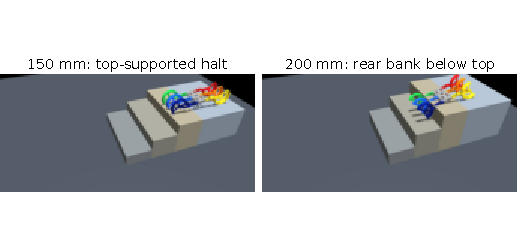
\includegraphics[width=\columnwidth]{stair_endpoint.pdf}
\caption{Terminal states for the fixed arc policy at nominal approach and 350 mm tread. Left: 150 mm ascent followed by a supported halt. Right: 200 mm timeout with incomplete rear-bank transfer. Both images are simulation, not physical validation.}
\label{fig:endpoint}\end{figure}

\subsection{Periodic Flat Control Remains Competitive}
All 176 flat trials complete their prescribed horizons. All 128 bounded-target trials satisfy issued-target and inner-profile rate bounds. Table~\ref{tab:flat} summarizes the high-command main comparison. P retains B's transport level across these settings; this result favors periodic scheduling for the evaluated flat task rather than adding conditional logic without demonstrated benefit.

\begin{table}[t]\centering\small
\caption{Mean flat speed at a 0.45 m/s command}
\label{tab:flat}\begin{tabular}{lccc}\toprule
Clock / rate scale & U & B & P\\\midrule
Unlimited & .287 & .289 & .289\\
H, $\rho=1.0$ & .220 & .223 & .224\\
H, $\rho=0.8$ & .231 & .227 & .228\\
F, $\rho=0.8$ & .320 & .316 & .317\\
H, $\rho=0.5$ & .136 & .145 & .146\\\bottomrule
\end{tabular}
\par\vspace{4pt}\noindent\parbox{\columnwidth}{\footnotesize Speeds in m/s; four paired phases and 20 s per trial. H waits for target issuance; F continues the gait clock. All cells complete 4/4 trials. The settings alter requested trajectories or their timing and do not represent equal tracking fidelity.}
\end{table}

For P under H at $\rho=0.8$, maximum requested-to-issued lag is $20.8^\circ$, compared with B's $30.0^\circ$. The worst observed joint tracking RMS is approximately $5.6^\circ$ for both. F produces faster transport, but changes the sequence of requested targets; it does not show that time scaling preserves the same motion at higher speed. Under H at $\rho=0.8$, the 60 s high-command means are 0.216 m/s for P and 0.216 m/s for B after rounding. These observations support simplification of the tested scheduling decision.

Command compliance is insufficient for physical feasibility. Across the flat study, actual joint speed reaches 1.23 times the declared command limit, loaded support can fall to one tire, and selected timestep pairs differ in speed by as much as 0.011 m/s. Root-velocity integration and displacement agree within $5.2\times10^{-5}$ m/s. These checks separate dynamic limitations from measurement consistency.

\section{DISCUSSION AND CONCLUSION}
The useful result is a separation of roles. Flat transport does not require conditional reindex scheduling in the tested cases. Stair ascent over the 100--150 mm grid does not require height-specific phase and posture selection. Contact shape has a larger effect on the main-grid completion count than the tested $15^\circ$ posture change, while posture can reduce ascent time and work without changing the success set. 

The evidence does not establish that all articulation can be removed. C180 still acquires and holds an articulated side-on posture; it is not a rigid-hip RHex or a six-motor hardware ablation. Nor does the comparison identify a unique hooking mechanism: the full arc-to-cylinder change also changes outer support, phase-dependent radius, and contact topology. Contact-event analysis and calibrated physical trials would be needed to distinguish those effects.

The 200 mm failure motivates testing a support-aware phase pause or scheduled posture change to transfer the rear bank, using the same completion rule and preparation accounting. This recovery extension remains untested.

Finally, the model uses rigid tires, disables most non-tire collision geometry, and omits hinge hard stops. It does not establish full-body clearance, tire compliance, loaded motor capability, or physical multi-turn feasibility. Archival stair and floor videos document embodiment under earlier controllers without synchronized logs. An uninterrupted floor--stair--floor experiment, matched physical shape/posture trials, and resolution of the wheel's timestep sensitivity remain necessary for a hardware mobility claim. The tested 100--150 mm conditions support a fixed policy; rear-bank transfer at 200 mm remains unresolved.

\section*{ACKNOWLEDGMENT AND AI DISCLOSURE}
OpenAI Codex assisted with drafting and revising all sections, implementing simulation and analysis scripts, and assembling figures from measured data and source media. Numerical results were produced by executing the archived experiment code. No generated photorealistic images are used as experimental evidence.
\bibliographystyle{IEEEtran}\bibliography{references}
\end{document}
